\documentclass[oneside,12pt]{amsart}
%included packages###############################################################
\usepackage{setspace}
\usepackage[english]{babel}
\usepackage{graphicx}
\usepackage{float}
\usepackage{tabularx}
\usepackage{mathtools}
\usepackage{mathrsfs}
\usepackage{amsfonts}
\usepackage{amssymb}
\usepackage{siunitx}
\usepackage{amsthm}
\usepackage{enumitem}
\usepackage{stmaryrd}
\usepackage{multirow}
\usepackage{parskip}
\usepackage{csquotes}
\usepackage{systeme}
\usepackage{caption}
\usepackage{cases}
\usepackage{algorithm}
\usepackage{algpseudocode}
\captionsetup[table]{position=bottom} %UNCOMMENT IF USING CAPTIONS, COMMENTED TO SUPPRESS WARNINGS
\usepackage[backend=biber,style=numeric]{biblatex} %UNCOMMENT IF USING BIBLIOGRAPHY, COMMENTED TO SUPPRESS WARNINGS
\addbibresource{Biblio.bib}
\usepackage[letterpaper, total={6in, 9in}]{geometry}
%Set up graphic path#########
\graphicspath{{./}{}}% You can add the path for the images in the empty brackets 

%Set document dimensions#########################################################
\newdimen\graph
\graph=4.2in
\newdimen\medgraph
\medgraph = 5.3in
\newdimen\smallgraph
\smallgraph = 3in
\newdimen\tinygraph
\tinygraph = 1.5in
\renewcommand{\arraystretch}{1.5}

%Define custom commands here#####################################################
\newcommand{\R}{\mathbb{R}}
\newcommand{\Z}{\mathbb{Z}}
\newcommand{\N}{\mathbb{N}}
\newcommand{\Q}{\mathbb{Q}}
\newcommand{\C}{\mathbb{C}}
\newcommand{\mb}{\mathbf}
\newcommand{\e}[1]{\hat{\mathbf{#1}}}
\newcommand{\esymb}[1]{\hat{\bm{#1}}}
\newcommand{\sub}[1]{_{\text{#1}}}
\newcommand{\lbl}[1]{\stepcounter{equation}\tag{\theequation}\label{#1}}

%Define Custom Operators here ##################################################
\DeclareMathOperator{\arctanh}{arctanh}
\DeclareMathOperator{\const}{const.}

%Define theorems here#################################################################

%Title info#######################################################
\title{A Fine-Grained analysis of XGBoost predicting $T_c$ }
\author{Daniel Briseno}
\date{}
%-Begin Document-%%%%%%%%%%%%%%%%%%%%%%%%%%%%%%%%%%%%%%%%%%%%%%%%%%%%%%%%%%%%%%%%%%%%%%%%%%%%%%%%%%%%%%%%%%
\begin{document}
\maketitle
\section{Introduction}
This project is a review of the ability of the XGBoost regression tree algorithm's ability to predict the critical temperature ($T_c$) of superconductors, as proposed by Dr. Hamdieh in \cite{hamidieh_data-driven_2018}.

In \cite{hamidieh_data-driven_2018}, Dr. Hamidieh reports that a properly optimized XGBoost model can give an out-of-sample residual mean squared error (RMSE) of approximately $9.5^\circ$ K. Here, I will present a finer grained analysis of the performance of XGBoost. More specifically, I will attempt to answer the following questions:
\begin{enumerate}
	 \item How well does XGBoost preform at predicting $T_c$ of Iron, Cuprate, Mercury and $\text{MgB}_2$ based super conductors? Does this performance improve or worsen when trained only on Iron, Cuprate, or $\text{MgB}_2$ based superconductors?
     \item If we divide the testing data by quartiles of $T_c$, how well does XGBoost preform at predicting $T_c$ of compounds in each quartile? Is XGBoost reliable when predicting the $T_c$ of a compound with a high $T_c$?
     \item If we divide the predictions of XGBoost by quartiles of predicted $T_c$, how accurate and precise is XGBoost's prediction when the prediction falls in a given quartile? Is the predicted value of $T_c$ reliable when this predicted value is high?
\end{enumerate}

\section{The Dataset}

The data used to train and test the XGBoost model both in \cite{hamidieh_data-driven_2018} and in this report is taken from the Superconductivity Dataset found in the UCI Machine Learning Repository\cite{noauthor_superconductivity_2018}. It is a collection of 21263 superconductors with 82 features defined for each superconductor. The 82nd feature is $T_c$ and will serves as the target label. The features of the superconductors are generated from atomic properties of the elements in the superconductor. These properties are summarized in Table \ref{tab:elemental_properties} (this table can also be found in \cite{hamidieh_data-driven_2018}).

  For a given superconductor in the data, the atomic properties of the elements which make up that superconductor are combined according to the summary statistics listed below:
 \begin{enumerate}
     \item Mean
     \item Weighted mean
     \item Geometric mean
     \item Weighted geometric mean
     \item Entropy
     \item Weighted entropy
     \item Range
     \item Weighted range
     \item Standard deviation
     \item Weighted standard deviation
 \end{enumerate}
 
 A more in-depth explanation of these summary statistics and their associated formulas can be found in Table 2 of \cite{hamidieh_data-driven_2018}. 
 
 
 \begin{table}[ht]
     \centering
     \tiny
     \begin{tabularx}{\linewidth}{X X X}
          \hline
          Variable & Units & Description\\
          \hline
        Atomic Mass &Atomic mass units (AMU) &Total proton and neutron rest masses\\
        First Ionization Energy &Kilo-Joules per mole (kJ/mol)&Energy required to remove a valence electron\\
        Atomic Radius & Picometer (pm) &Calculated atomic radius\\
        Density&Kilograms per meters cubed (kg/m3)&Density at standard temperature and pressure\\
        Electron Affinity &Kilo-Joules per mole (kJ/mol) &Energy required to add an electron to a neutral atom\\
        Fusion Heat &Kilo-Joules per mole (kJ/mol) &Energy to change from solid to liquid without temperature change\\
        Thermal Conductivity &Watts per meter-Kelvin (W/(m K)) &Thermal conductivity coefficient $\kappa$\\
        Valence &No units &Typical number of chemical bonds formed by the element\\
        \hline
     \end{tabularx}
     \caption{Elemental properties used to define features used by XGboost to predict $T_c$. }
     \label{tab:elemental_properties}
 \end{table}
 
 \section{Methods}
  In this section I will describe the data collection process by first specifying the error statistics collected for predicted $T_c$ values, then describing how these error statistics were collected for any relevant subset of the training and testing data, then finally describing the subsets themselves.
 
 \subsection{Error Statistics}
 
 Let $P$ be the predicted value of $T_c$ and $A$ be the actual value. Then I define the \textbf{raw error} $err$ as $err := P-A$. Note that a negative raw error indicates an under-prediction, and a positive raw error indicates an over-prediction.
 
 This investigation consisted of collecting summary raw error statistics for $T_c$ predictions by XGBoost on relevant subsets of the testing and training data. The error statistics collected are summarized in Table \ref{tab:err_stats}.
 
 \begin{table}[ht]
     \centering
     \begin{tabularx}{\linewidth}{X X}
     \hline
     Statistic & Description\\
     \hline
       RMSE & The residual mean squared error of predictions \\
        ave\_err  & Raw average of error\\
        std\_err & Standard deviation of raw error values\\
        under\_cnt & Number of under-predictions\\
        over\_cnt & Number of over-predictions\\
        correct\_cnt & Number of exactly correct predictions. Expected to be 0\\
        ave\_under & Average value of under-prediction raw error\\
        ave\_over & Average value of over-prediction raw error\\
        std\_under & Standard deviation of under-prediction raw error\\
        std\_over & Standard deviation of over-prediction raw error\\
        \hline
     \end{tabularx}
     \caption{Summary error statistics collected for predicted $T_c$ values.}
     \label{tab:err_stats}
 \end{table}
 
 \subsection{Subsets Studied}
 Previously, I introduced three questions concerning the performance of XGBoost across three categories: superconductors containing certain elements, superconductors in different true $T_c$ quartiles, and superconductors in different predicted $T_c$ quartiles. 
 
 To this end, there are three classes of subsets under consideration: the element subsets, the true $T_c$ quartiles, and the predicted $T_c$ quartiles.
 
 \subsubsection{The Element Subsets}
 There were four subsets of the data which I call the element subsets. These subsets are: superconductors containing Fe (Iron), containing Cu (Copper), containing $\text{MgB}_2$, and containing Hg (Mercury).
 
 The motivation for the Fe, Cu, and $\text{MgB}_2$ subsets is the body of previous work which applied machine learning to predicting $T_c$ for superconductors containing these compounds. Predicting $T_c$ for superconductors containing these compounds has received priority in the literature due to the practical applications of such superconductors. Thus, it would be useful to characterize how well XGBoost performs on these superconductors.
 
 The motivation for the Hg subset comes from the distribution of $T_c$ values for all superconductors in the dataset, summarized in Figure \ref{fig:Tc_density}. This distribution is extremely skewed towards low values, and is not particularly clustered around a mean. Thus, it seems possible that the model would be biased towards low $T_c$ values. Superconductors containing Hg offer a ``worst case" analysis. Not only do these superconductors have the highest mean $T_c$ of any other elemental class in the dataset, they also have the fourth highest variance \cite{hamidieh_data-driven_2018}. 
 
 \begin{figure}[ht]
     \centering
     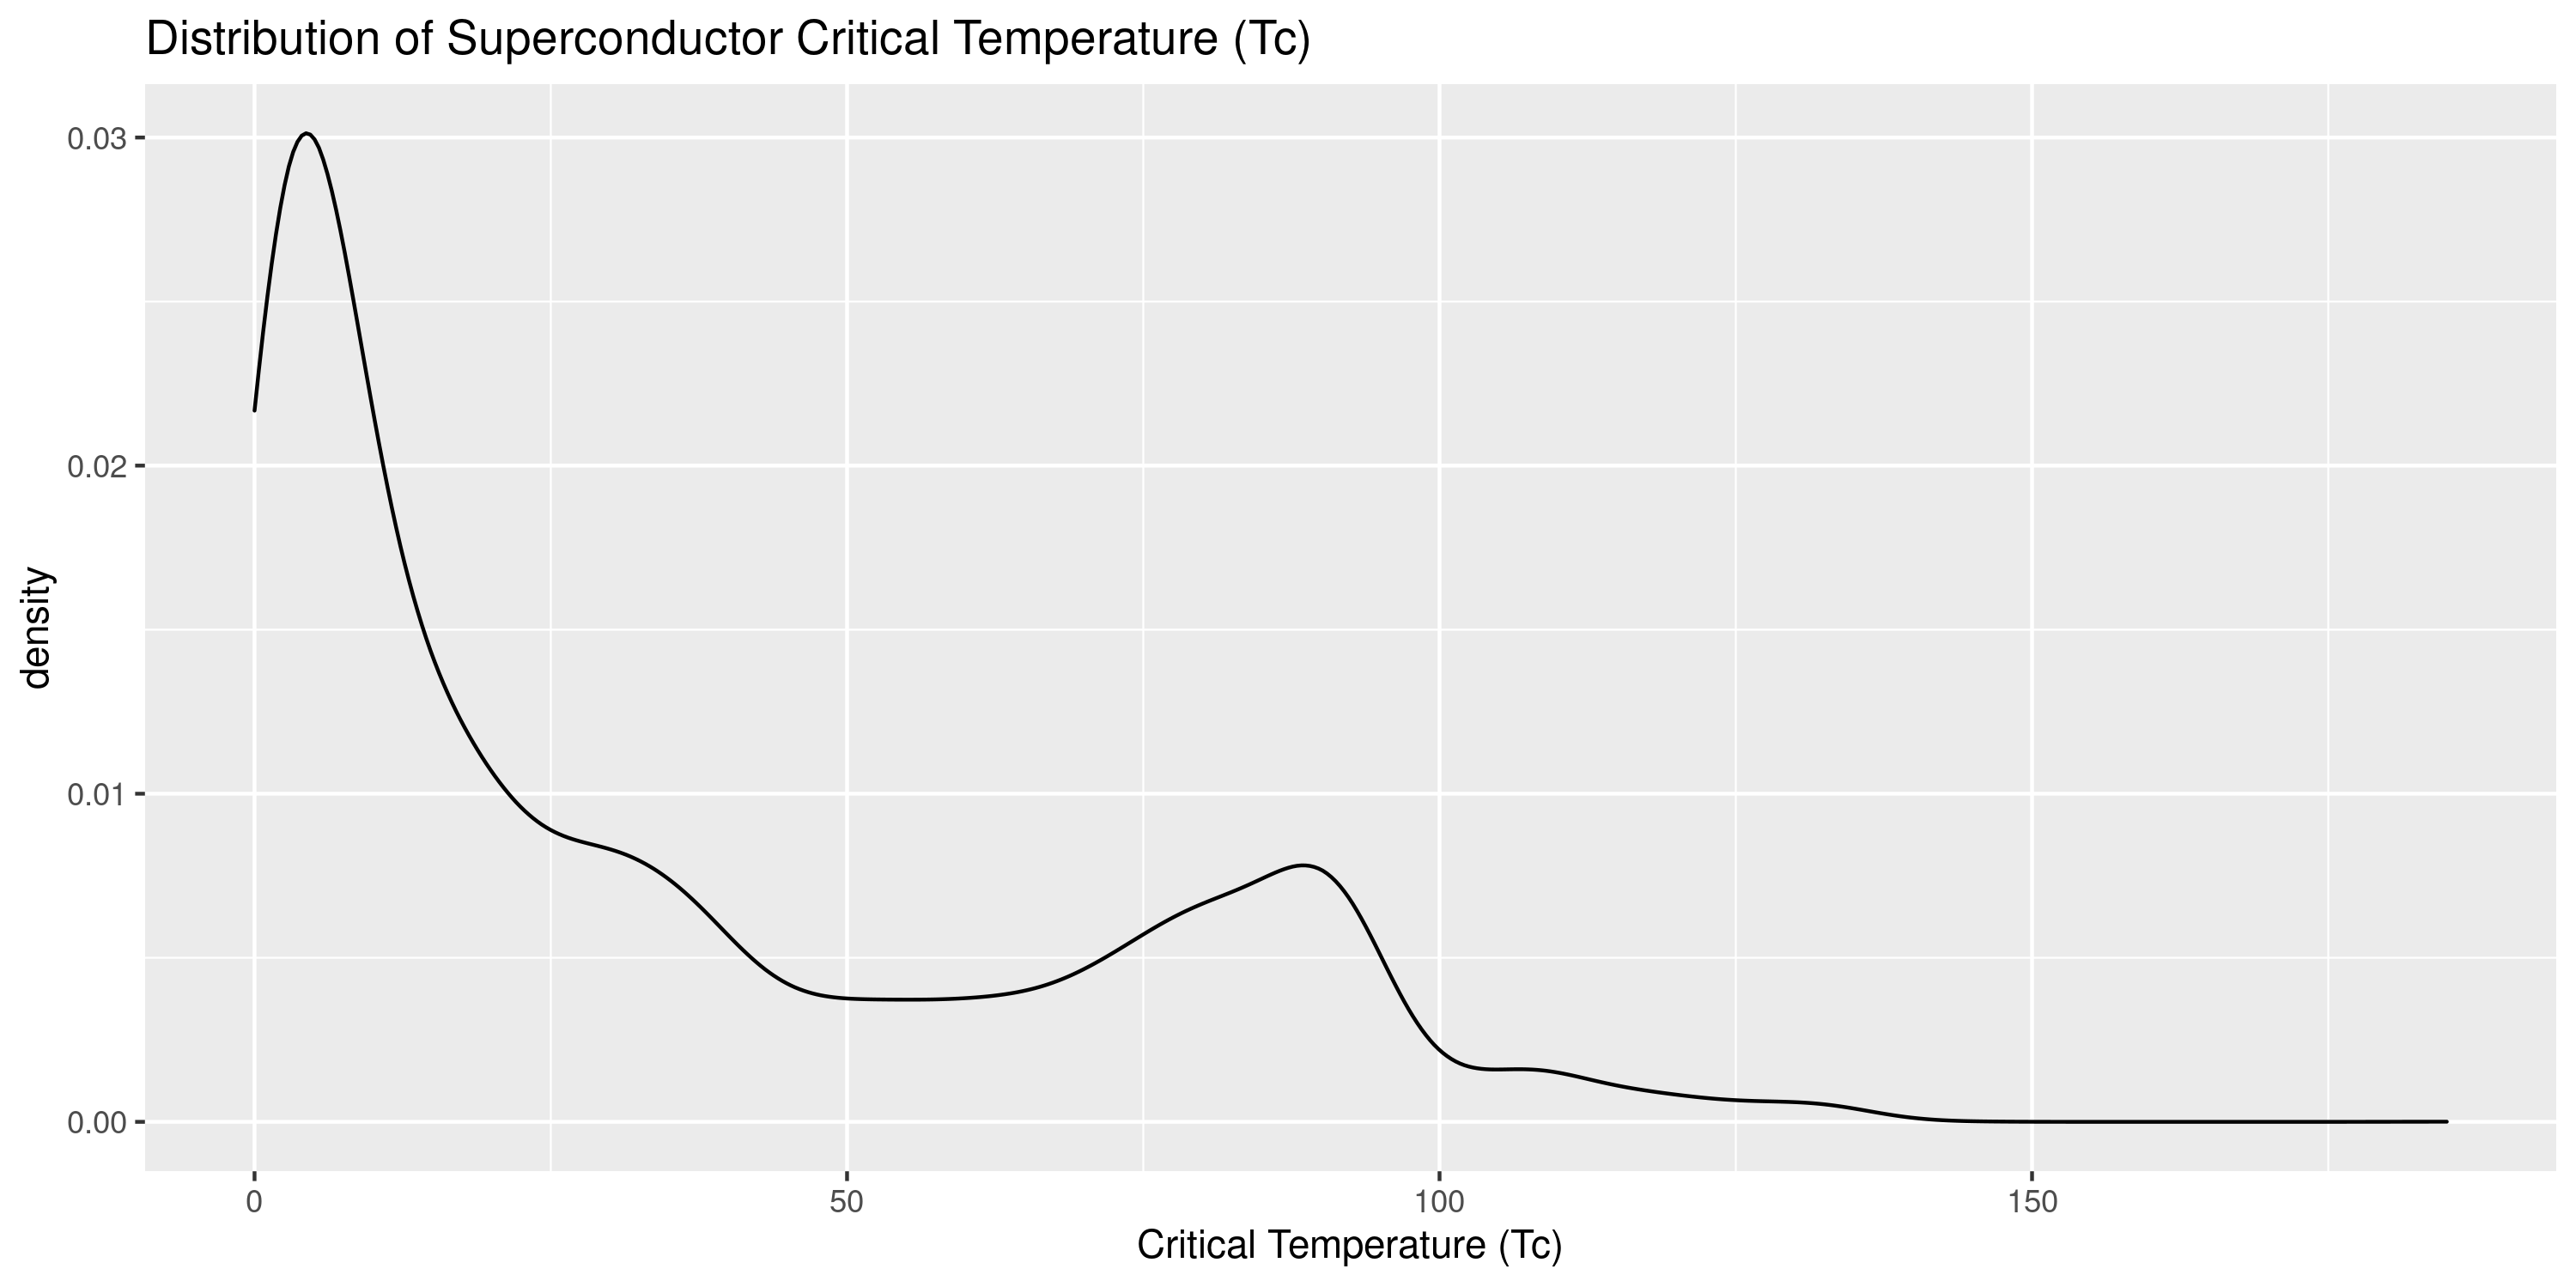
\includegraphics[width=0.8\linewidth]{../Plots/Tc_dist.png}
     \caption{Density plot of $T_c$ values for all superconductors in dataset.}
     \label{fig:Tc_density}
 \end{figure}
 
 Besides determining the performance of XGBoost on these four subsets, we will analyze any potential benefits of training XGBoost only on compounds of a given element subset when trying to predict $T_c$ values for that subset. The motivation for this is to determine if it would be useful to have separate models for these subsets (as has been done in literature previous to \cite{hamidieh_data-driven_2018}), or if the more generalizable XGBoost model trained on the entire training data gives accurate enough predictions.
 
 Thus, there are two different test conditions for the element subsets.
 \begin{enumerate}
 \item No Retrain: The XGBoost model will be trained on an unrestricted random partition of the data.
 \item Retrain: The XGBoost model will be trained only on superconductors belonging to a single element subset.
 \end{enumerate}
 
 \subsubsection{The True $T_c$ Quartiles}
 As one would expect, these subsets are divided by $T_c$ quartile. The motivation for these subsets is again the distribution of $T_c$ values. Since the distribution is skewed towards low values, it is likely that the algorithm under-predicts values in the upper quartiles. 
 
 Identifying this under-prediction (or any other systematic error) may lead to a better optimized algorithm which takes a likely under-prediction of certain superconductors into account.
 
 \subsubsection{The Predicted $T_c$ Quartiles}
 These subsets are the superconductor quartiles, where each superconductor is placed in a quartile according to its \textit{predicted} $T_c$ value. The motivation for this subset is identical to the motivation for the true $T_c$ quartiles, with one distinction. With the predicted $T_c$ quartiles, we will take into account the fact that we do not know the true $T_c$ of an arbitrary conductor. Because of this, implementing a correction term based off of true $T_c$ values would prove difficult, if not impossible.
 
 If a systematic errors can be identified within the predicted $T_c$ quartiles, then implementing a correction term would be easy. We would only need to pick the suitable correction term based off of the observed predicted value of $T_c$.
 
 \subsubsection{Control Data} We will also analyze the performance of XGBoost on a simple 2/3 training and 1/3 testing partition of the superconductor data. 
 
 \subsection{Collection of Error Statistics}
The collection of error statistics was as follows:
\begin{enumerate}
	\item The dataset described in section 2 is split into 2/3 training data 1/3 testing data.
	\item The model is trained and tested on the corresponding partitions, and residuals are taken for each prediction on the testing data.
	\item Summary statistics of the residuals are taken over the classes of superconductors described in 3.2.
\end{enumerate}
In the case of the retraining condition on the element subsets, an additional step is added before step (1), where the entire dataset is partitioned into element subsets, and steps (1)-(3) proceed using a single element subset.

\section{Results}

\subsection{Results on the Control Data}

 Figure \ref{fig:control_table} presents average error statistics from the 50 error vectors collected for the control data. Note that the average RMSE is of about $9.5^\circ$ K, thus we can confirm the out-of-sample RMSE presented in \cite{hamidieh_data-driven_2018}.
 
 \begin{figure}[ht]
     \centering
     
\includegraphics[width = \linewidth]{../Plots/control_tbl.png}
     \caption{Average error statistics from 50 random test/train splits.}
     \label{fig:control_table}
 \end{figure}


Moreover, we see that we have a mean error near 0, and a standard deviation of error nearly equal to the RMSE. This is characteristic for normally distributed residuals, and indicates that the RMSE can be attributed to random error, rather than a bias in the model.

 \begin{figure}[ht]
     \centering
     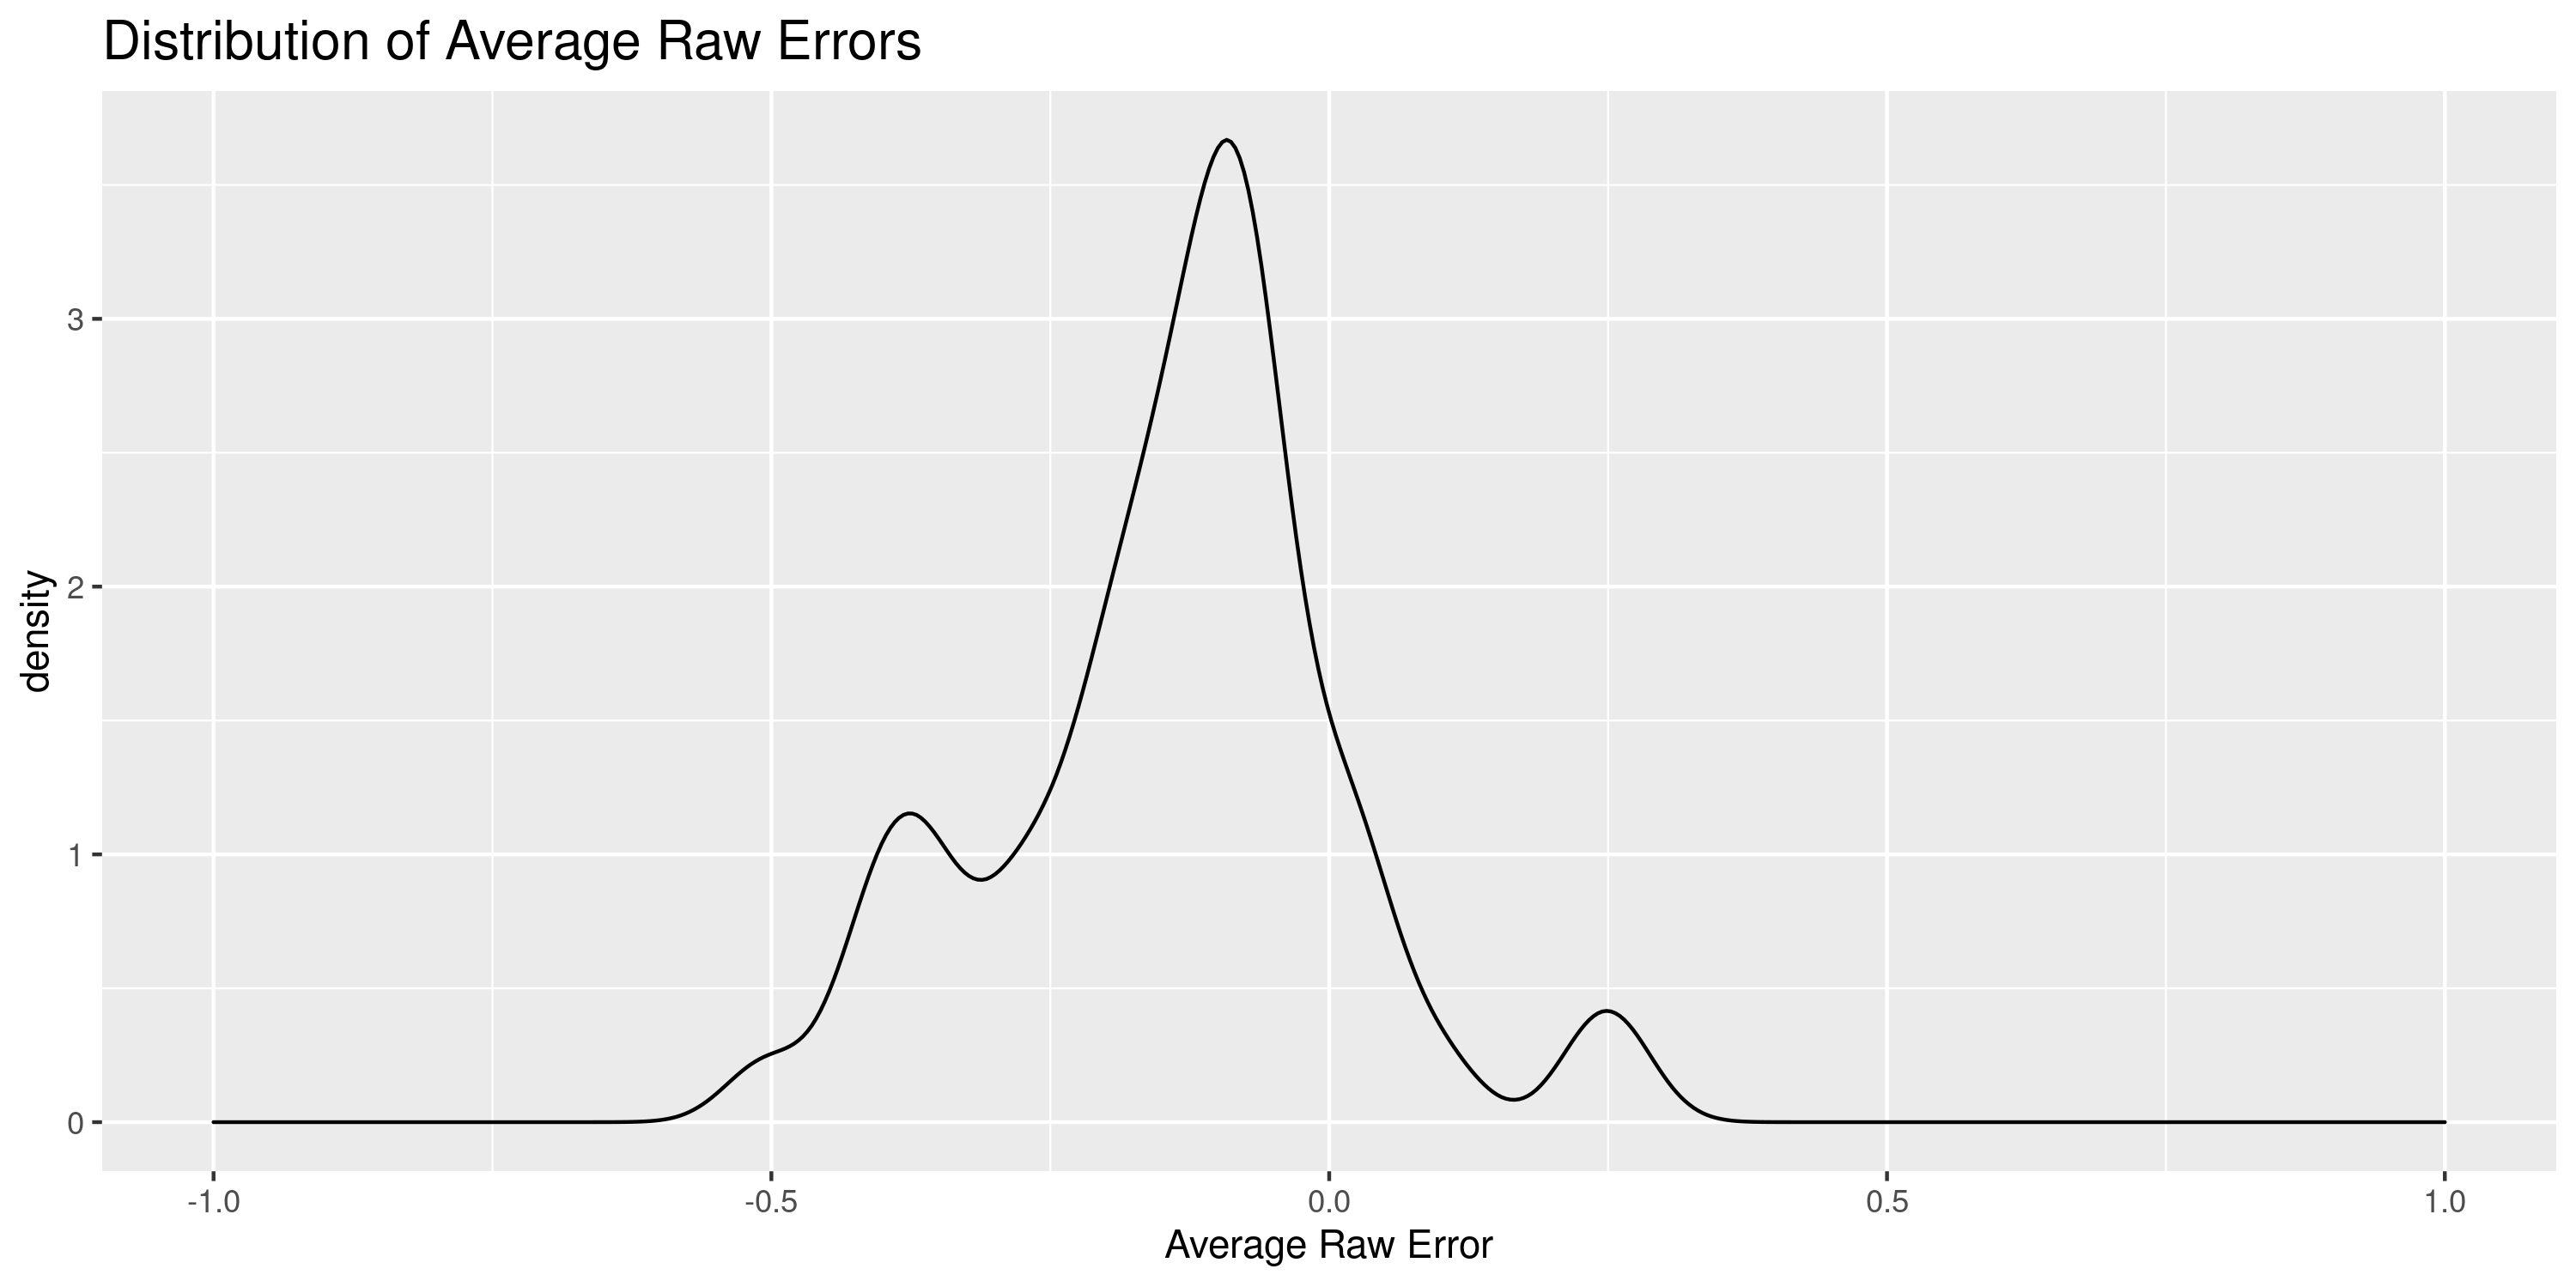
\includegraphics[width=0.8\linewidth]{../Plots/control_ave_err_density.png}
     \caption{Density plot of average raw errors. Raw error averages were taken from 50 random train/test splits.}
     \label{fig:err_denisty}
 \end{figure}

By plotting the average raw error from 50 random train/test splits in Figure \ref{fig:err_denisty}, we do see that the model has a slight under-prediction bias, since the distribution of average errors is skewed towards the left. This is not surprising, since the distribution of superconductor critical temperature is heavily skewed towards low critical temperatures (as seen in Figure \ref{fig:Tc_density}).


\begin{figure}[ht]
    \centering
    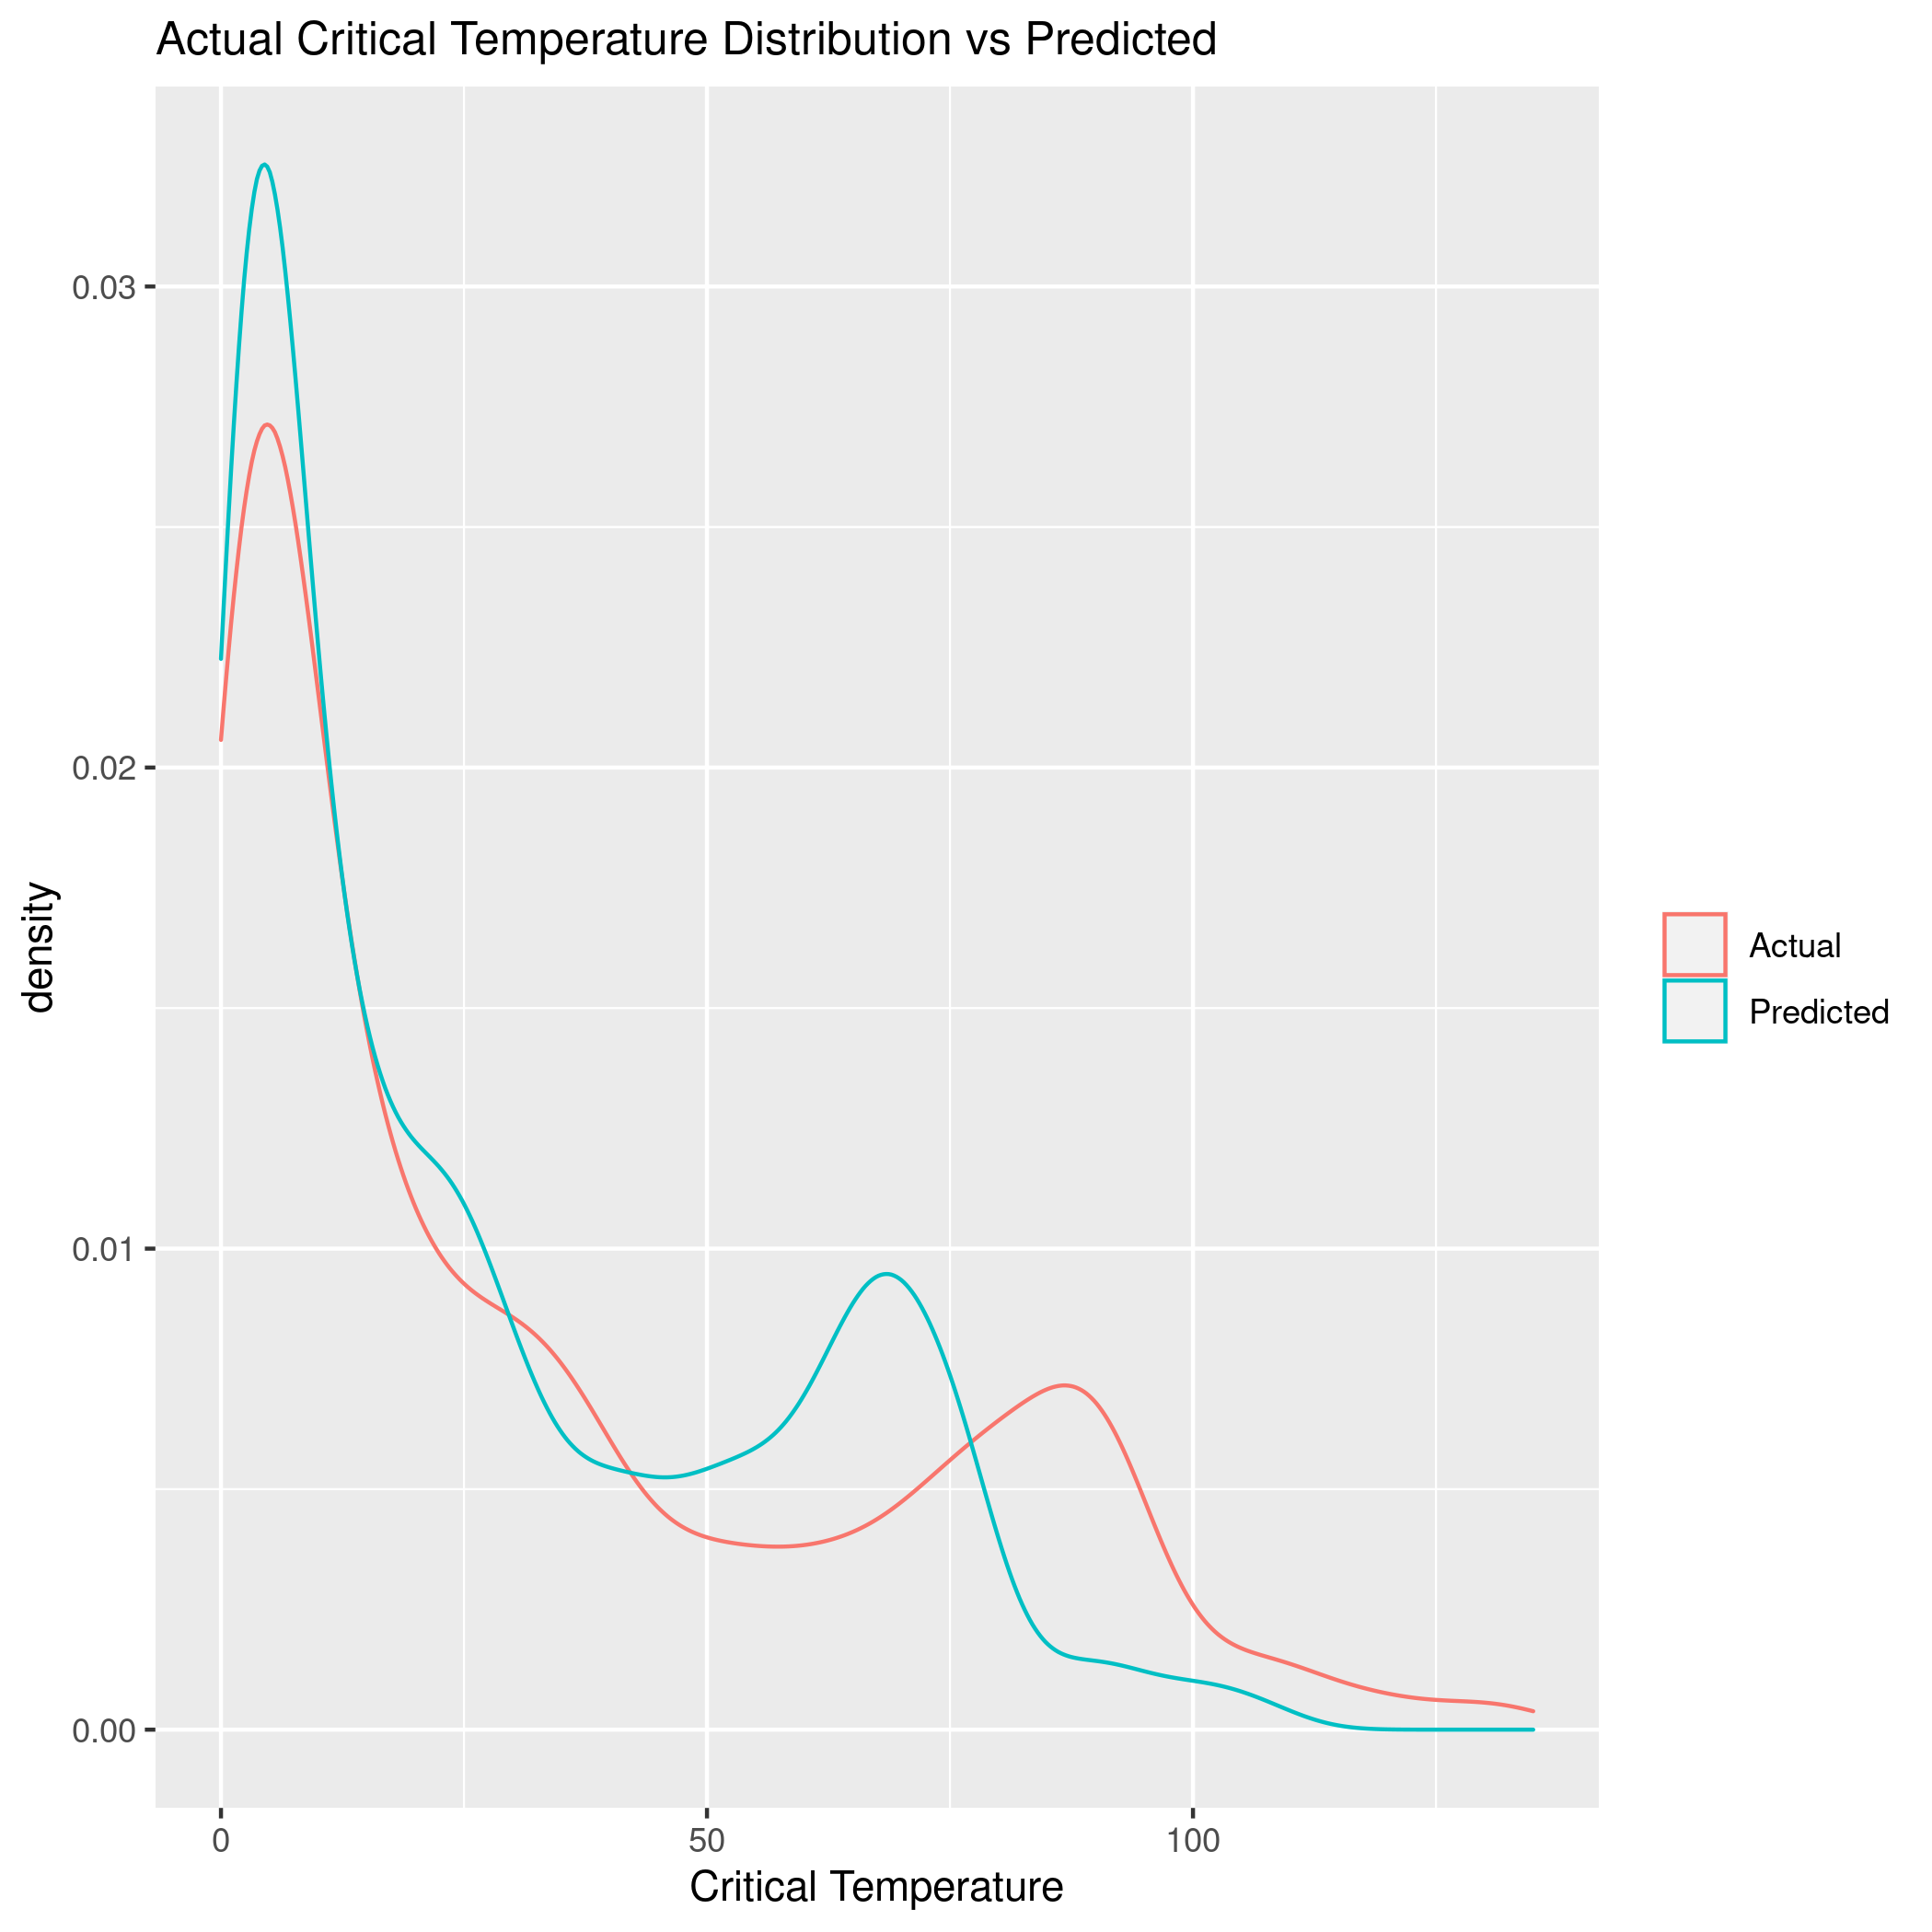
\includegraphics[width=0.8\linewidth]{../Plots/Actual_vs_Pred_dist.png}
    \caption{Actual test partition $T_c$ distribution plotted alongside the predicted $T_c$ distribution. }
    \label{fig:actual_vs_pred_Tc_dist}
\end{figure}
 
Figure \ref{fig:actual_vs_pred_Tc_dist} more clearly shows the nature of the slight under-prediction bias. In particular we see that:
\begin{enumerate}
     \item XGBoost correctly finds a sharp peak in the distribution of $T_c$ values near a temperature of $0^\circ$ K. However, the model slightly over-estimates the number of superconductors present in this low $T_c$ cluster.
     \item XGBoost correctly identifies a second smaller peak in the distribution with high $T_c$ values. However, XGBoost over-estimates the number of superconductors present in this high $T_c$ cluster, and slightly under-estimates the temperature at which this cluster occurs.
 \end{enumerate}
 
\subsection{Results on the Element Subsets}

 
 Figure \ref{fig:elemental_ntr_tbl} presents average error statistics for the 4 element subsets when XGBoost is trained on a random train partition in the data. Thus, the XGBoost model used to collect these error statistics can be taken to be identical to the model in the control data section.
 
 \begin{figure}[ht]
     \centering
     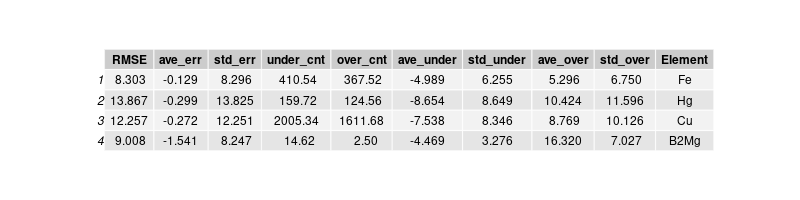
\includegraphics[width = \linewidth]{../Plots/element_no_retrain_tbl.png}
     \caption{Average error statistics from 50 error vectors per element subset.}
     \label{fig:elemental_ntr_tbl}
 \end{figure}
 
As expected, we see that the model performed worst on superconductors containing mercury, with a RMSE of 13.867. None of the element subsets show a clear prediction bias towards high or low $T_c$ predictions, with the possible exception of $\text{B}_2\text{Mg}$ based superconductors. The model under-predicted $T_c$ for these superconductors approximately six times more times than it over-predicted. However, we can also see that this element subset had a very small sample size, which is the likely source of the poor predictions.

 \begin{figure}[ht]
     \centering
     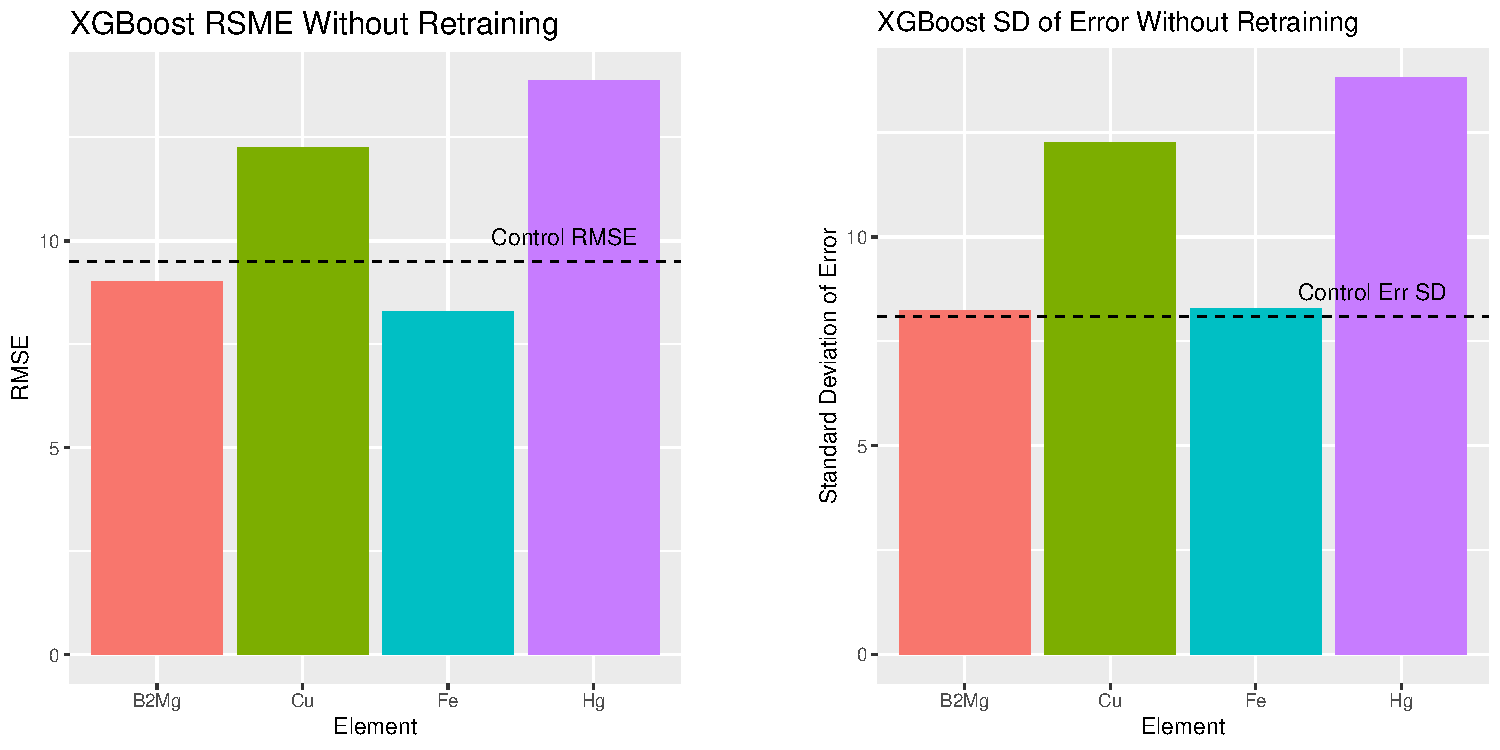
\includegraphics[width=\linewidth]{../Plots/Element_ntr_brplt.pdf}
     \caption{RMSE and standard deviation of error on the element subsets without retraining XGBoost on the element subsets. The RMSE and standard deviation of error for the control data are indicated with dashed lines.}
     \label{fig:elemental_nrt_comparsion}
 \end{figure}
 
Initially, I had suspected that superconductors containing Hg would have a severe under-prediction bias, since Hg containing superconductors have the highest average $T_c$. However, we do not see this bias, as the average error is near zero and we see that the number of under predictions is nearly the same as the number of over predictions.


  \begin{figure}[ht]
     \centering
     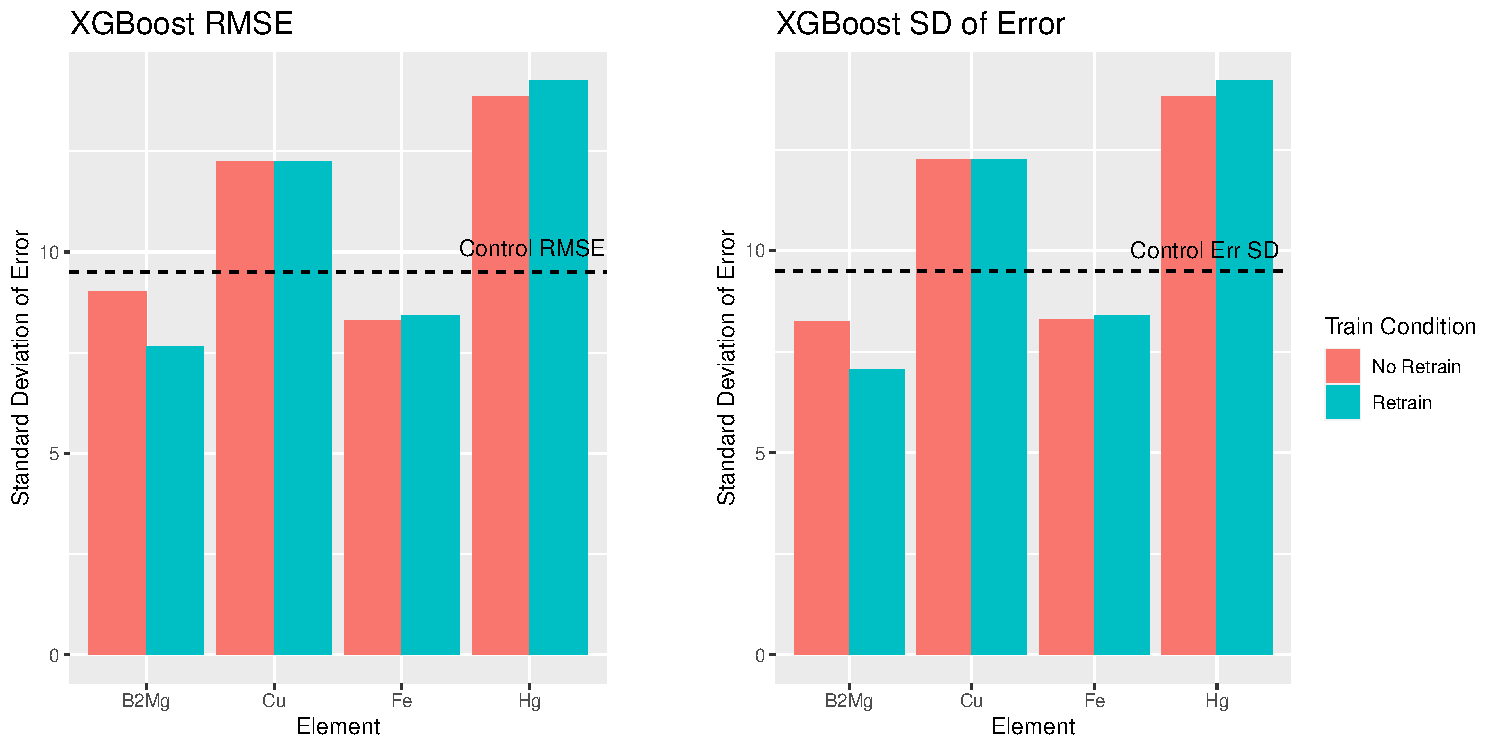
\includegraphics[width=\linewidth]{../Plots/Element_comparison_bxplt.pdf}
     \caption{Comparison of RMSE and Standard deviation between retraining and no-retraining conditions}
     \label{fig:elemental_rt_brplt}
 \end{figure}
 

The overall performance of the model on the element subsets is better seen in Figure \ref{fig:elemental_nrt_comparsion}. Here, we can clearly see that the model performed worse on copper and mercury containing superconductors than the reported RMSE of 9.5 in \cite{hamidieh_data-driven_2018}. Moreover, we can see that this poorer performance is likely due to random error in the model's predictions rather than some correctable bias, since the standard deviation of the prediction residuals closely mirrors the RSME.

It is important to note that while the RMSE is up to $4^\circ$K higher in the element subsets than in the control data, the distribution of superconductor $T_c$ ranges from nearly $0^\circ$K to $150^\circ$K. Thus, the model predicts $T_c$ reasonably well across all element subsets.
 
\begin{figure}
     \centering
     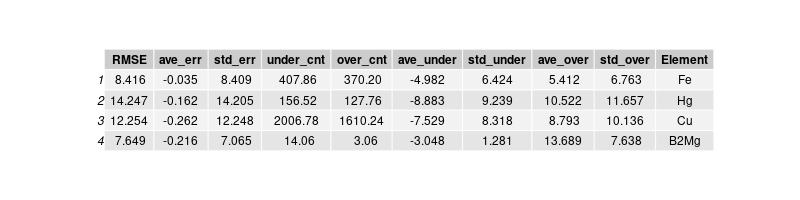
\includegraphics[width = \linewidth]{../Plots/element_retrain_tbl.png}
     \caption{Average error statistics from 50 error vectors per element subset. In this case, XGBoost was retrained on the elemental subsets.}
     \label{fig:elemental_rt_tbl}
 \end{figure}

Figure \ref{fig:elemental_rt_brplt} shows that retraining the model on only superconductors belonging to the elemental subset on which it is tested on did not improve the performance of XGBoost. It is interesting to note that the model's performance in both the Retrain and No Retrain conditions was very similar, despite drastic changes to the training data. I believe that this might be due to the the fact that XGBoost is a gradient boosted decision tree algorithm. Thus, by reducing the training sample to only the element subsets, we may have simply re-created the portions of the decision trees in XGBoost which lead to a prediction for superconductors containing Fe, Cu, Mg or $\text B_2\text{Mg}$.

\subsection{Results on the True $T_c$ Quartiles}

 \begin{figure}
     \centering
     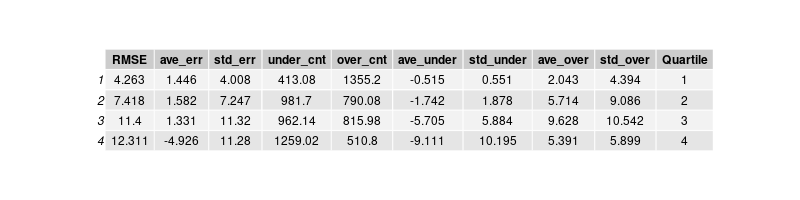
\includegraphics[width = \linewidth]{../Plots/quartile_true_tbl.png}
     \caption{Average error statistics from 50 error vectors collected for each true $T_c$ quartile.}
     \label{fig:quart_true_ave_tbl}	
 \end{figure}
 
 Figure \ref{fig:quart_true_ave_tbl} presents average error statistics for the 4 true $T_c$ quartiles. While the model performs reasonably well across all quartiles, we can see that the model performs best for superconductors with low $T_c$, and worse on superconductors with a high $T_c$. 
 
 This is not ideal, since the primary use-case of this model would be to find a superconductor with a high $T_c$. However, Figure \ref{fig:quart_true_ave_tbl} suggests that the XGBoost model is likely to under-predict the critical temperature of such a material.
 

 \begin{figure}
     \centering
     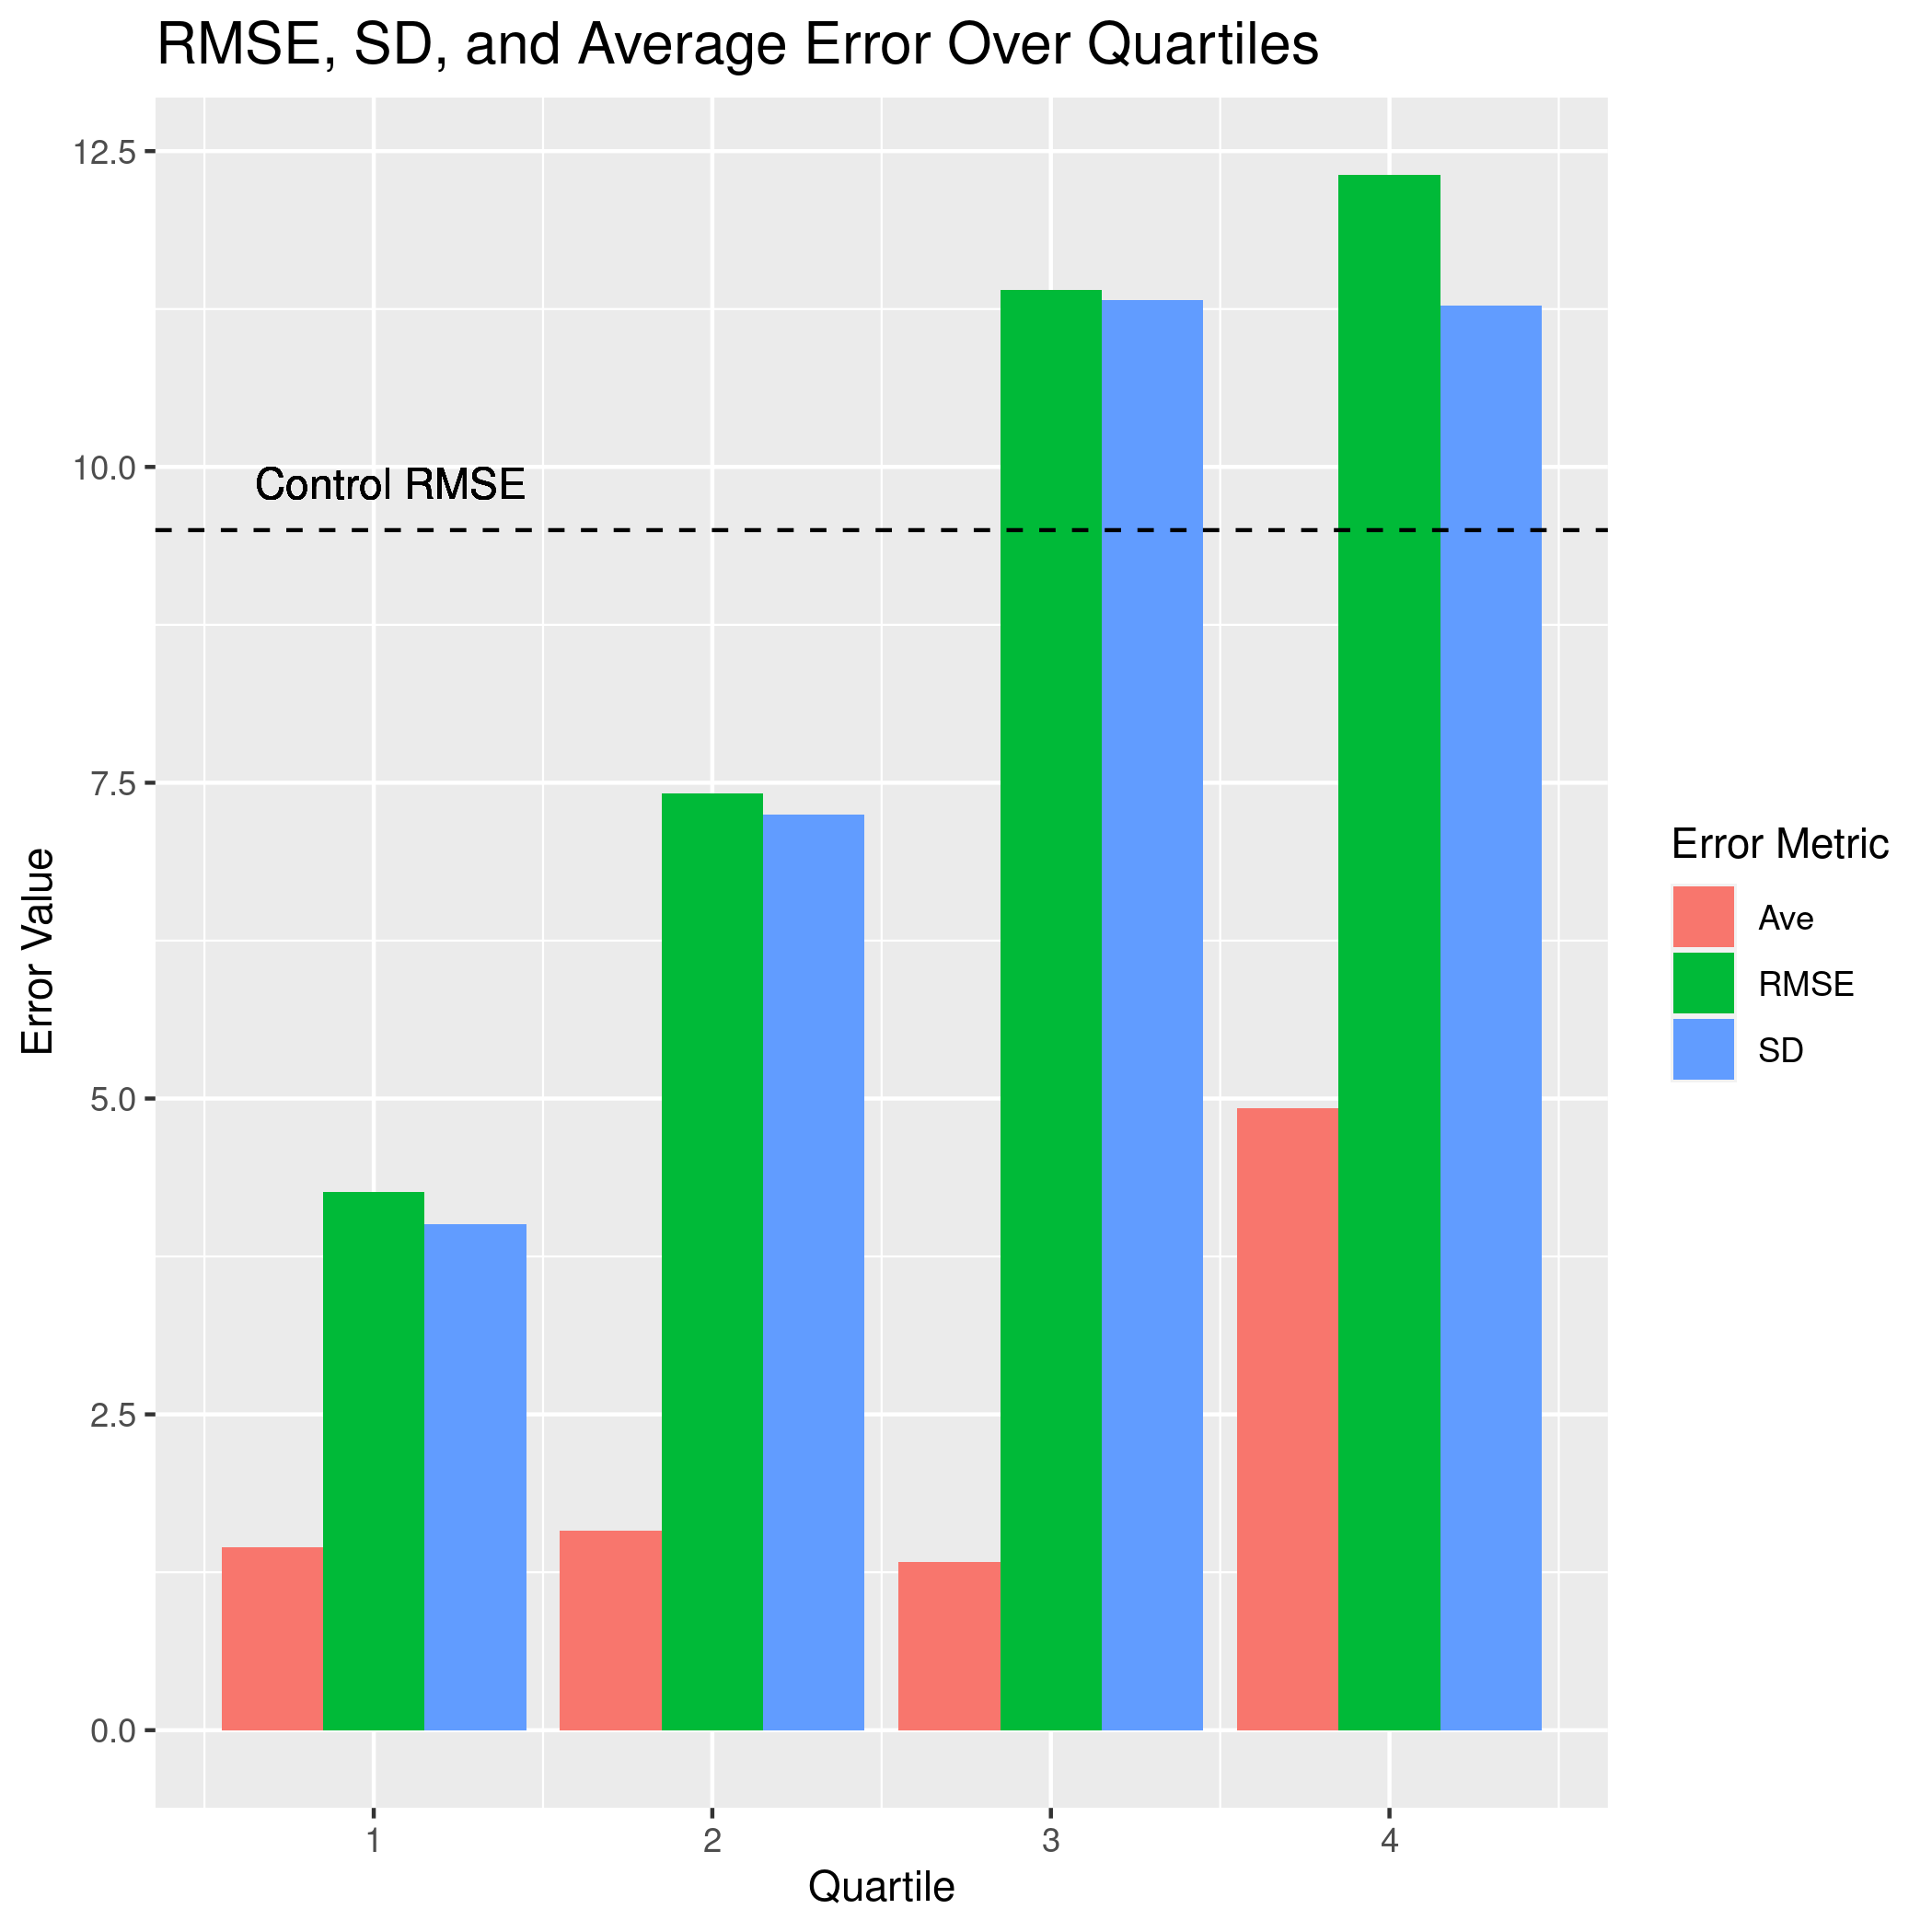
\includegraphics[width=0.8\linewidth]{../Plots/True_Q_error_brplt.png}
     \caption{RSME, standard deviation of error, and the average of raw errors plotted alongside each other for each true $T_c$ quartile.}
     \label{fig:True_Q_Ave_brplt}
 \end{figure}
  
   However, by looking at the average error, we see that for the 4th quartile, the model has a $-5^\circ$ K bias. Thus, it might be possible to correct for under predictions in the 4th quartile, and so slightly improve the performance of the model in this quartile.
 
\subsection{Results on the Predicted $T_c$ Quartiles}
Of course, we cannot know in which $T_c$ quartile a superconductor with an unknown $T_c$ will belong. Thus, I investigated if this bias is still present if each superconductor is placed in a quartile based off of its \textit{predicted} $T_c$.


\begin{figure}
    \centering
    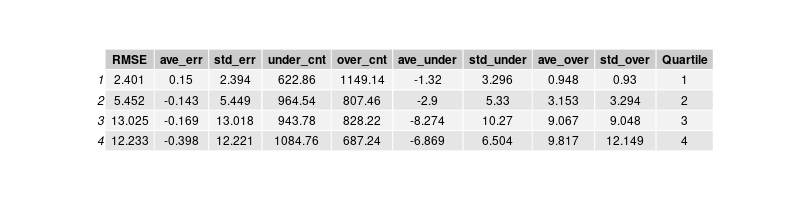
\includegraphics[width=\linewidth]{../Plots/quartile_pred_tbl.png}
    \caption{Average error statistics from 50 error vectors collected for each predicted $T_c$ quartile.}
    \label{fig:quart_pred_ave_tbl}
\end{figure}

\begin{figure}
    \centering
    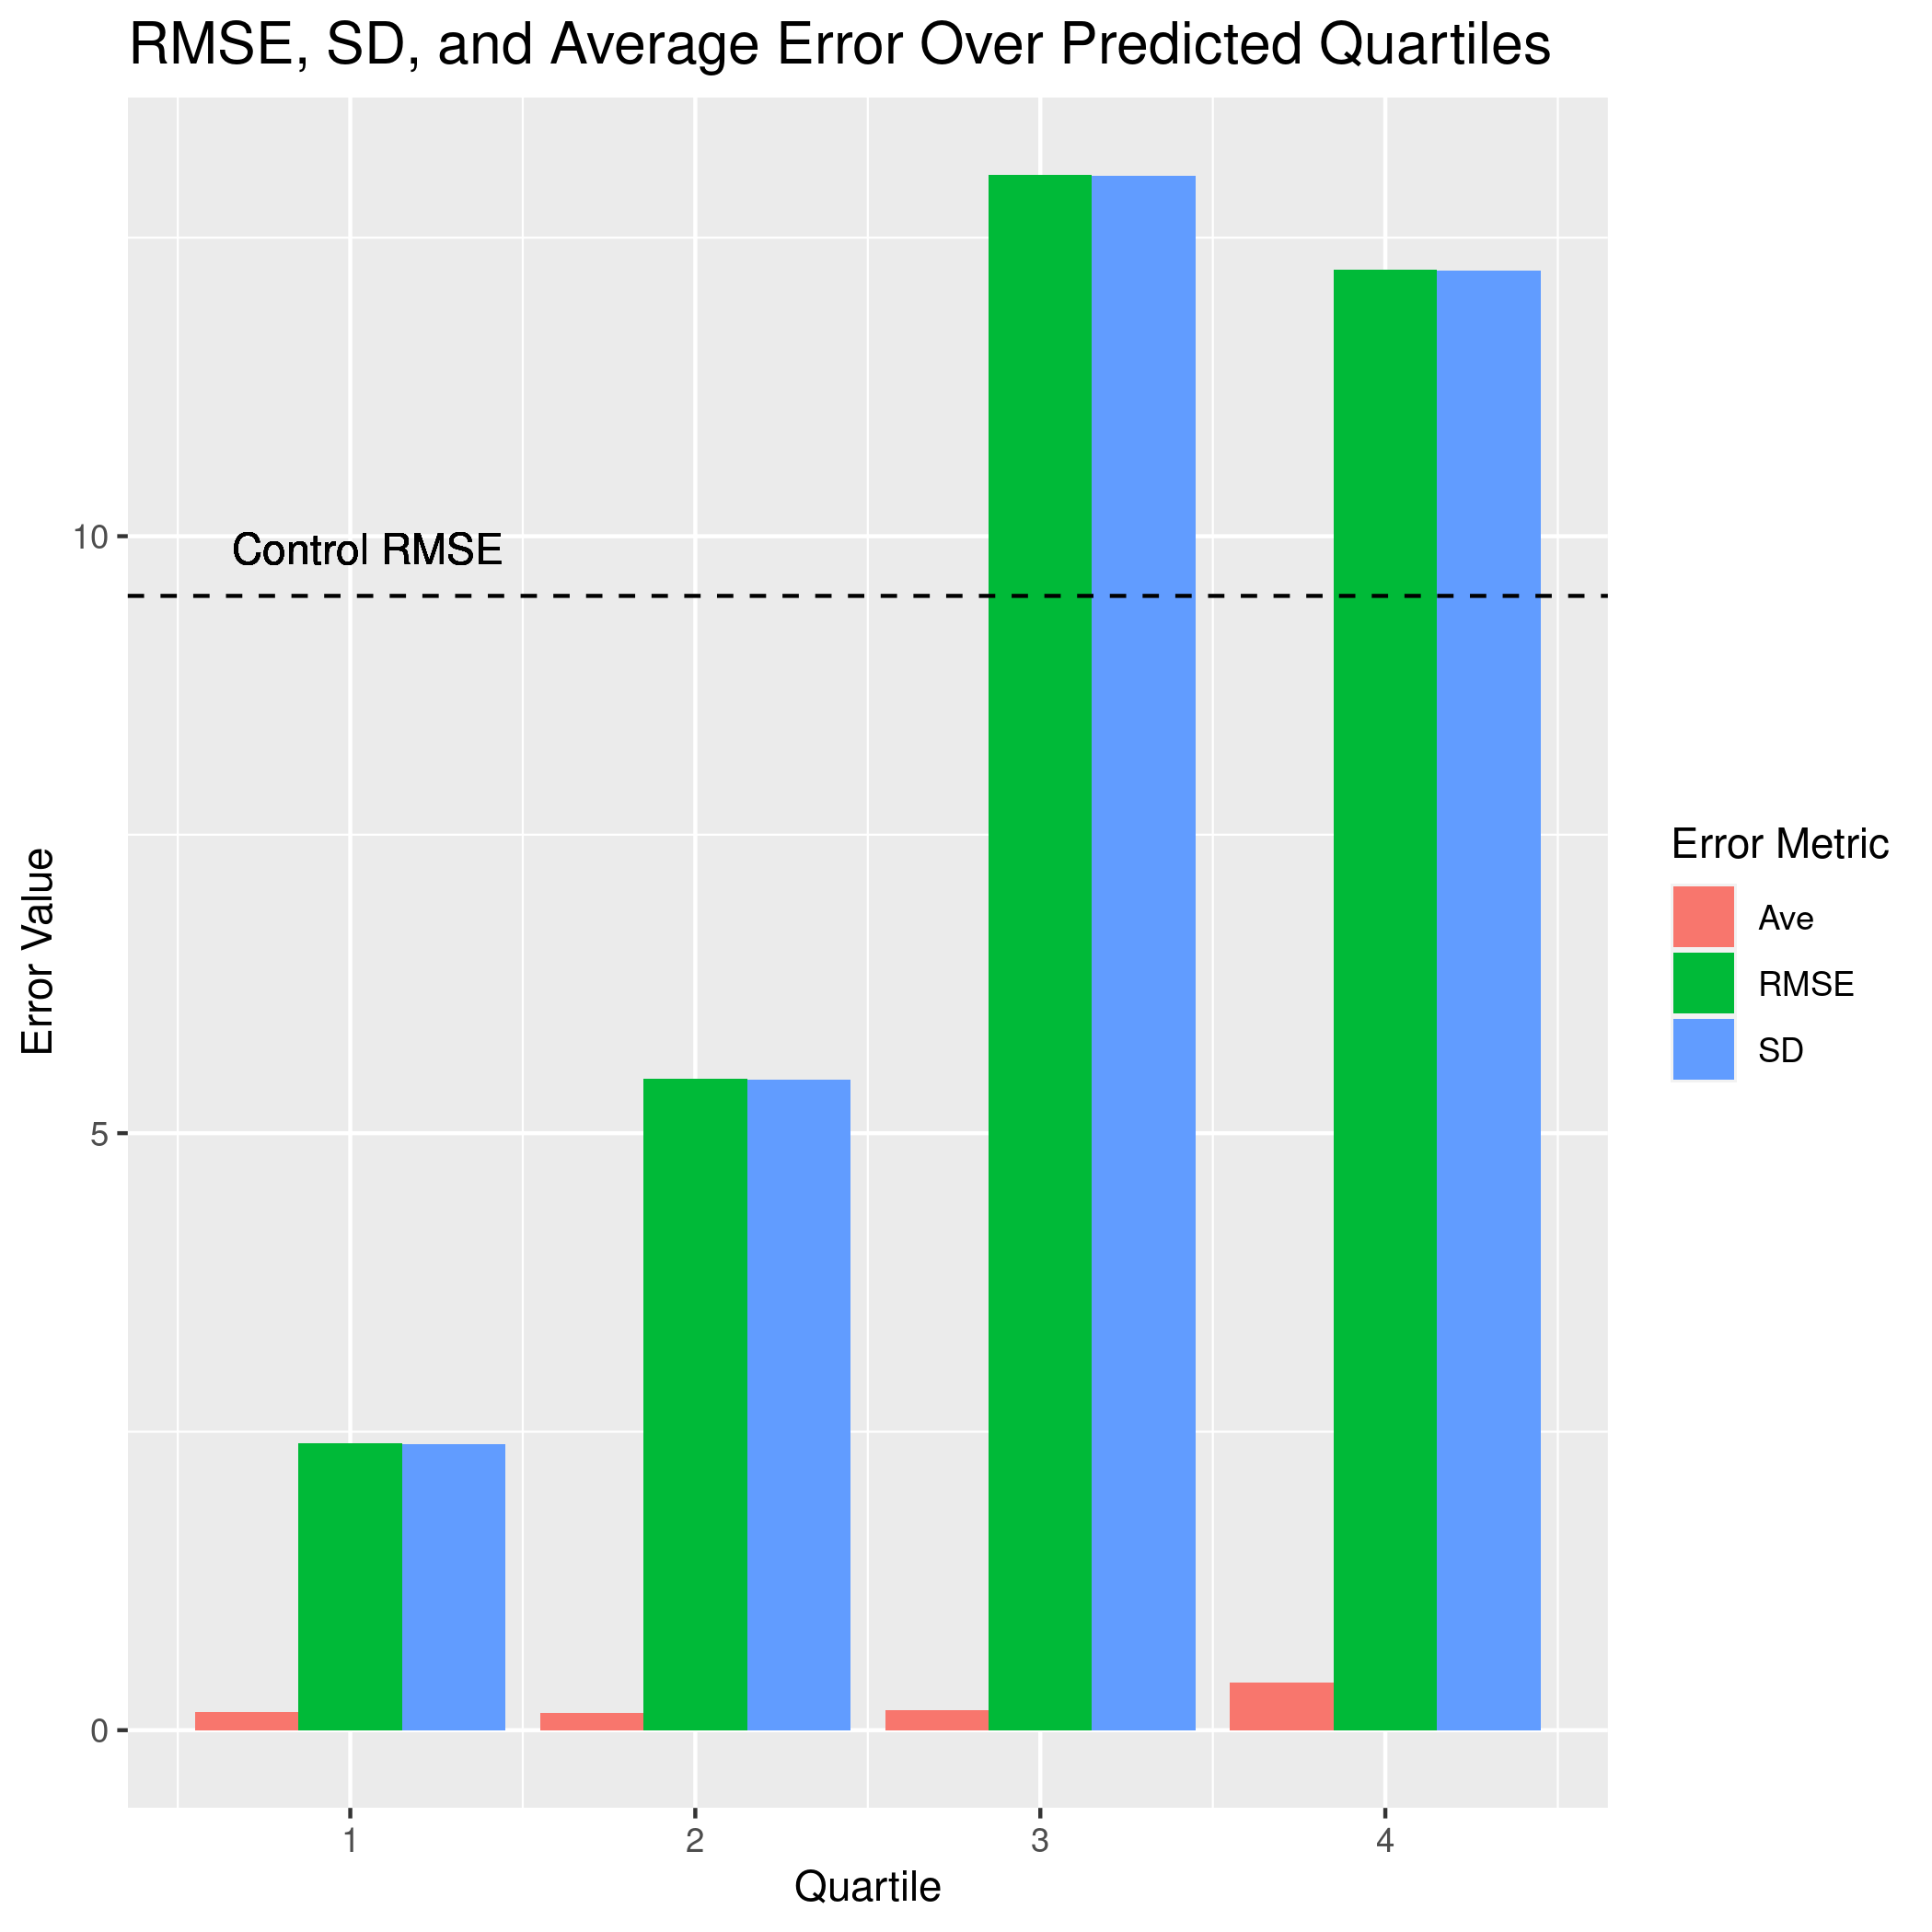
\includegraphics[width = 0.7\linewidth]{../Plots/Pred_Q_error_brplt.png}
    \caption{RMSE, standard deviation of error, and the average of raw error plotted alongside each other for each predicted $T_c$ quartile.}
    \label{fig:Pred_Q_Ave_brplt}
\end{figure}

Unfortunately, Figures \ref{fig:quart_pred_ave_tbl} and \ref{fig:Pred_Q_Ave_brplt} show that this is not the case. While we still see that the performance of the model worsens in the higher quartiles, there is no bias in the predictions for any quartile. 

Interestingly, we see that the RMSE in the 3rd quartile was higher than in the 4th. This may be due to the fact that superconductors belonging to the 4th true $T_c$ quartile are mistakenly predicted to belong in the 3rd quartile, due to the under prediction bias we had seen earlier. Thus, the 3rd quartile is likely to contain many superconductors with under predicted $T_c$. 

\section{Conclusion}

In this report, we analyzed the performance of XGBoost across three categories of superconductors in order to answer the following three questions:

 \begin{enumerate}
     \item How well does XGBoost preform at predicting $T_c$ of Iron, Cuprate, Mercury and $\text{MgB}_2$ based super conductors? Does this performance improve or worsen when trained only on Iron, Cuprate, or $\text{MgB}_2$ based superconductors?
     \item If we divide the testing data by quartiles of $T_c$, how well does XGBoost preform at predicting $T_c$ of compounds in each quartile? Is XGBoost reliable when predicting the $T_c$ of a compound with a high $T_c$?
     \item If we divide the predictions of XGBoost by quartiles of predicted $T_c$, how accurate and precise is XGBoost's prediction when the prediction falls in a given quartile? Is the predicted value of $T_c$ reliable when this predicted value is high?
 \end{enumerate}
 We are now in a position to provide answers to these three questions:
 
 \begin{enumerate}
     \item XGBoost predicts $T_c$ for Iron, Cuprate, and Mercury based superconductors reasonably well; in each case XGBoost predicts $T_c$ with an RMSE nearly equal to the RMSE of $T_c$ predictions for the control data ($9.5^\circ$ K), but was higher than the control RMSE for cuprate and mercury based superconductors. The performance of XGBoost at predicting $T_c$ for these subsets does not significantly change when using training data only from these subsets.
     \item XGBoost preforms reasonably well across all quartiles, but RMSE does increase for increasing $T_c$ quartiles. Thus, the XGBoost model presented in \cite{hamidieh_data-driven_2018} is reliable for predicting the critical temperature of materials in the 4th quartile, but less reliable than it would be for lower quartiles. This increase in RMSE is partially driven by an increase in prediction bias in the 4th quartile, with XGBoost consistently under predicting $T_c$ in this quartile.
     \item As observed in the true $T_c$ quartiles, XGBoost performs with decreasing accuracy for increasing $T_c$ quartiles, but is still reasonably accurate. Thus, the model is reasonably reliable when the predicted $T_c$ value is high. Unlike for the true $T_c$ quartiles, there is no observable bias in the predictions for the 4th predicted $T_c$ quartile.
 \end{enumerate}
 
\newpage
\printbibliography
\end{document}